\model{Class Diagram}

\begin{multicols}{2}

Recall that a UML class diagram summarizes the attributes and methods of a class.
In the repair shop example, a \java{Car} class might look something like this:

\columnbreak
\centering

\vspace*{-4.5em}
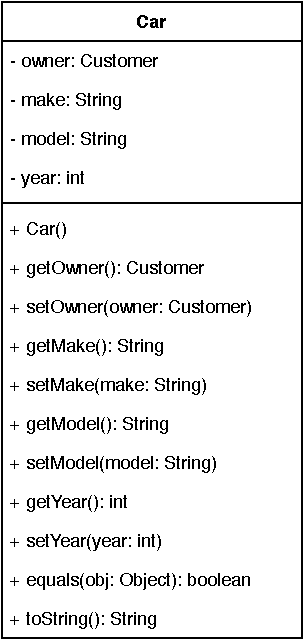
\includegraphics[scale=1]{Car-UML.pdf}

\end{multicols}


\quest{15 min}


\Q How many \blank\ are in the diagram above?

\begin{multicols}{2}
\begin{enumerate}[itemsep=1ex]
\item attributes \ans[3em]{4}
\item constructors \ans[3em]{1}
\item getters \ans[3em]{4}
\item setters \ans[3em]{4}
\end{enumerate}
\end{multicols}


\Q What is the type of the \java{owner} attribute? Is it a primitive or reference type?

\begin{answer}[2em]
It is a \java{Customer}, or more specifically, a reference to a \java{Customer} object.
\end{answer}


\Q Explain how this design allows multiple cars to be owned by the same customer.

\begin{answer}[2em]
Multiple \java{Car} objects can reference the same \java{Customer} object in memory.
\end{answer}


%\newpage
%\comment{In the following questions, you will design the \java{Customer} class for the repair shop software.}


\Q List three attributes that would be appropriate for the \java{Customer} class.

\begin{center}
\begin{tabularx}{38.5em}{L{8.5em}|L{8.5em}|X}
Variable Name       & Data Type          & Example Value                    \\
\hline
\ans[8em]{name}     & \ans[8em]{String}  & \ans[18em]{"Jonathan Alger"}     \\
\ans[8em]{address}  & \ans[8em]{String}  & \ans[18em]{"800 S Main St ..."}  \\
\ans[8em]{phone}    & \ans[8em]{String}  & \ans[18em]{"(540) 568-6211"}     \\
\end{tabularx}
\end{center}


\Q Rewrite the attributes from the previous question in UML format.

\begin{answer}
- name: String \\
- address: String \\
- phone: String
\end{answer}


\Q \label{key2}
For each attribute, define a \java{get} method. Write your answer in UML format.

\begin{answer}
+ getName(): String \\
+ getAddress(): String \\
+ getModel(): String
\end{answer}


\Q \label{key3}
For each attribute, define a \java{set} method. Write your answer in UML format.

\begin{answer}
+ setName(String name) \\
+ setAddress(String address) \\
+ setModel(String model)
\end{answer}


\vfill
\subsection*{Optional Questions}


\Q What rules might be implemented in the \java{set} methods to ensure that only valid attribute values are stored?
\textit{Example: The customer's name should contain only letters and spaces.}

\begin{center}
\begin{tabularx}{38.5em}{L{8.5em}|X}
Variable Name       & Validation Rules                                               \\
\hline
\ans[8em]{name}     & \ans[27.5em]{no special characters, max length (e.g., of 50)}  \\
\ans[8em]{address}  & \ans[27.5em]{use an API like Google Maps to ensure it exists}  \\
\ans[8em]{phone}    & \ans[27.5em]{must be 10-digit number; use parens and dashes}   \\
\end{tabularx}
\end{center}


\Q Based on the attributes you defined, how could you determine whether two \java{Customer} objects represent the same customer?

\begin{answer}
Answers will vary.
It's probably good enough to compare the name and phone number.
But that would require names and numbers to be stored in a consistent format.
A more reliable approach would be to define a unique customer number.
\end{answer}


\Q In \ref{\currfilename}, what is the parameter name and type for the \java{equals} method?
What version of \java{equals} is this method overriding?

\begin{answer}
The name is \java{obj}, and the type is \java{Object}.
The \java{Car} class is overriding the default version of \java{equals} defined in the \java{Ojbect} class.
\end{answer}
